\documentclass[a4paper, 11pt,oneside]{article}
\usepackage[
  top=1.5cm,
  bottom=1cm,
  left=2cm,
  right=1.5cm,
  headheight=25.22153pt, % as per the warning by fancyhdr
  includehead,includefoot,
  heightrounded, % to avoid spurious underfull messages
]{geometry} 

\usepackage[T1]{fontenc}
\usepackage{microtype}
\usepackage{fancyhdr}
\usepackage{fancyvrb}
\usepackage{lipsum}
\usepackage{url}
\usepackage{listings}
\usepackage{lastpage}
\usepackage{enumitem}
\usepackage{datetime}
\usepackage{amsthm}
\usepackage{graphicx}
\usepackage{hyperref}
\usepackage{minted}
\usepackage{float}

\settimeformat{hhmmsstime}
\yyyymmdddate

\pagestyle{fancy}
\fancyhf{} % clear all fields

\pagestyle{fancy}
\lhead{CMSC 132: Computer Architecture \\ First Semester 2020-2021}
\rhead{Institute of Computer Science \\ University of the Philippines Los Banos}
\rfoot{JACHermocilla (CC NC-BY-SA 4.0)}
%\cfoot{Enjoy!:)}
\cfoot{\thepage\ of \pageref{LastPage}}
\lfoot{Revision: \today\ \currenttime}
%\rfoot{https://jachermocilla.org/teaching/125}
\renewcommand{\headrulewidth}{0.4pt}
\renewcommand{\footrulewidth}{0.4pt}

\begin{document}

\begin{center}
	{\LARGE \textbf{Combinational Logic Circuits}}
\end{center}

\section*{Learning Outcomes}
   At the end of this activity, you should be able to:
   \begin{enumerate}[itemsep=0pt,parsep=0pt]
   	   \item differentiate combinational and sequential elements in a processor;
       \item implement combinational logic circuit elements in VHDL;

   \end{enumerate}   

\tableofcontents

\section{Resources}
\begin{itemize}
	\item Video: \href{https://youtu.be/H2TmmSFds-M}{https://youtu.be/H2TmmSFds-M}.
	\item Source Codes: \href{https://git.io/JU3al}{https://git.io/JU3al}
\end{itemize}	


\section{Discussion}
The discussion in this handout aims only to provide an outline of what is in the video lecture. It is recommended that you watch the video in its entirety.

The computer can only execute machine language that it understands. This language is part of its architectural design or the Istruction Set Architecture (ISA). Machine language is nothing more than an encoding of bits. The computer can will do nothing unless instructions are given to it. These instructions will come from programmers. However, it is very difficult for programmers to use machine language directly. Assembly language is instead used which is more comprehensible for humans. The assembler translates the assembly language program to machine language. 

\subsection{Definitions}
Here are some terms worth knowing and remembering in this lab.

\begin{itemize}
	\item{\textit{Datapath} - The component of the processor that performs arithmetic operations}

	\item{\textit{Control} - The component of the processor that commands the datapath, memory, and I/O devices according to the instructions of the program}

	\item{\textit{Combinational elements} - Logic elements in the datapath that operate on data values}

	\item{\textit{State elements} - contains state, has some internal storage}

	\item{\textit{Edge-triggered clocking} - that any values stored in a sequential logic element are updated only on a clock edge, which is a quick transition from low to high or high to low}

	\item{\textit{Clock cycle length} - time to propagate the signal from state element 1, through the combinational element, and state element 2}

\end{itemize}

\subsection{Single-Cycle Datapath and Control}
A processor is composed of the datapath and control unit. Figure \ref{fig:datapath} shows an example of a 
single-cycle datapath and control. The main functional units are the following:
\begin{itemize}
	\item{\textit{Program Counter (PC)} - holds the address of the next instruction to be executed}
	\item{\textit{Instruction Memory (IM)}-holds the instructions/machine language}
	\item{\textit{Register File (RF)}- fast storage}
	\item{\textit{Arithmetic and Logic Unit (ALU)}- performs computations}
	\item{\textit{Data Memory (DM)}- holds data used by programs}
	\item{\textit{Control Unit (CU)}- drives the execution }
\end{itemize}

\begin{figure}[H]
	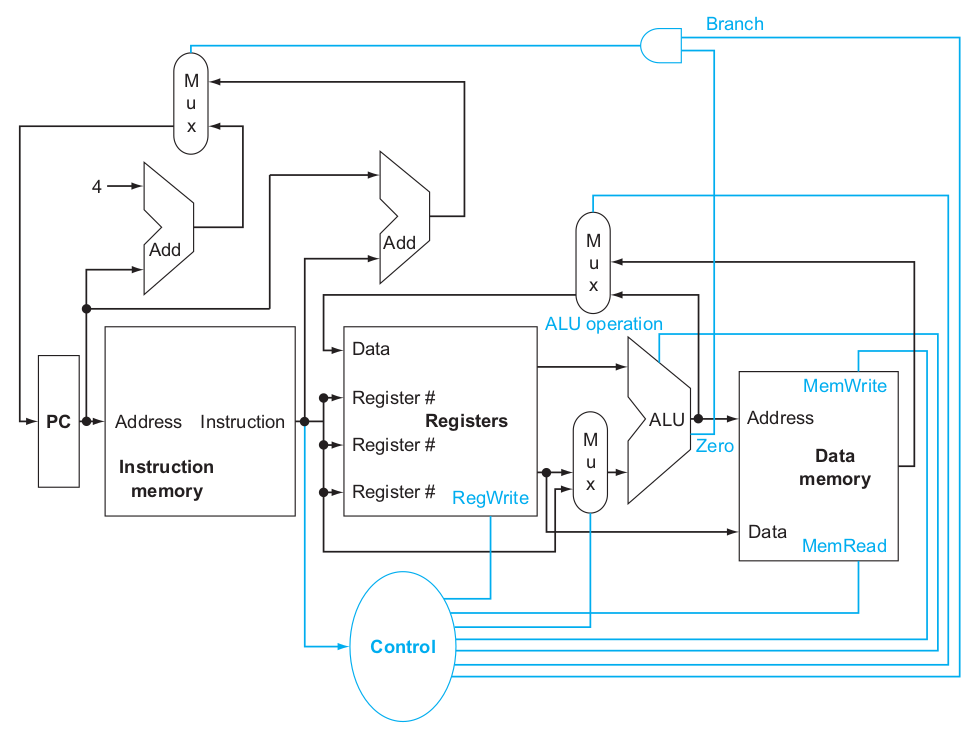
\includegraphics[width=\linewidth]{single-cycle-dp-control.png}
	\caption{Single-Cycle Datapath and Control.}
	\label{fig:datapath}
\end{figure}

The blue lines indicate control signals most of which originate from control based on the instruction being executed. You can think of the Control Unit as the 'brain' and the rest as the body parts.

Each of the above functional components are implemented using combinational and sequential logic circuits as building blocks. 

Instruction execution follows the following cycle or states:

\begin{itemize}
	\item {\textit{Instruction Fetch (IF)} - instruction is fetch from IM at address specified by PC}
	\item {\textit{Instruction Decode (ID)} - current instruction is examined for opcode and operands }
	\item {\textit{Execute (EX)} - perform operations based on opcode}
	\item {\textit{Memory (MEM)} - need to store data to DM}
	\item {\textit{Writeback (WB)} - result will be used stored in register or used in the next instruction}
\end{itemize}


\subsection{Decoders}
A decoder accepts an n-bit input and produces 2$^n$ outputs but only one output is asserted. Figure \ref{fig:decoder} shows an example 3-to-8 decoder. The VHDL implementation is also given below.


\begin{figure}[H]
	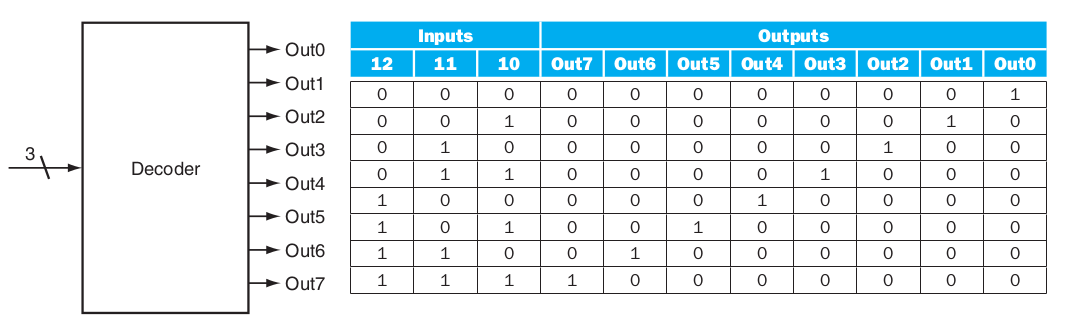
\includegraphics[width=\linewidth]{decoder.png}
	\caption{3-to-8 decoder.}
	\label{fig:decoder} 
\end{figure}

\begin{minted}[frame=single,framesep=10pt]{vhdl}
LIBRARY ieee;
USE ieee.std_logic_1164.all;
---------------------------------
ENTITY decoder_3to8 IS
   PORT (
      I2, I1, I0: IN STD_LOGIC;
      Out7, Out6, Out5, Out4, Out3, Out2, 
         Out1, Out0: OUT STD_LOGIC
   );
END decoder_3to8;
--------------------------------
ARCHITECTURE pure_logic OF decoder_3to8 IS
BEGIN
   Out0 <= NOT I2 AND NOT I1 and NOT I0;
   Out1 <= NOT I2 AND NOT I1 and I0;
   Out2 <= NOT I2 AND I1 and NOT I0;
   Out3 <= NOT I2 AND I1 and I0;
   Out4 <= I2 AND NOT I1 and NOT I0;
   Out5 <= I2 AND NOT I1 and I0;
   Out6 <= I2 AND I1 and NOT I0;
   Out7 <= I2 AND I1 and I0;
END pure_logic;
\end{minted}


\subsection{Multiplexers/Selectors}
A multiplexer select which input will be allowed to pass through as output. Figure \ref{fig:mux} show a mux with the selecter \textit{S} and two inputs \textit{A} and \textit{B}. It is implemented using two AND gates and one OR gate. To support multiple bits, this single bit multiplexer can be cascaded as an array as shown in Figure \ref{fig:mux_bits}.

\begin{figure}[H]
	\begin{center}
	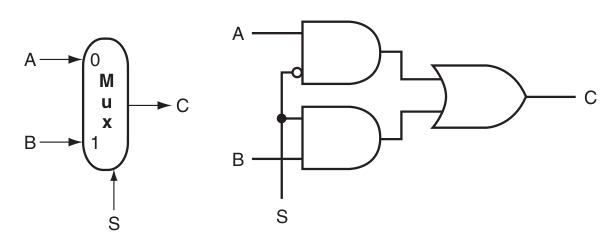
\includegraphics[width=4in]{mux.png}
	\caption{2-to-1 Multiplexer.}
	\label{fig:mux} 
	\end{center}
\end{figure}

The VHDL code for the 2-to-1 multiplexer is shown below.
\begin{minted}[frame=single,framesep=10pt]{vhdl}
LIBRARY ieee;
USE ieee.std_logic_1164.all;
---------------------------------
ENTITY mux_2to1 IS
   PORT (A, B, S: IN STD_LOGIC;
   C: OUT STD_LOGIC);
END mux_2to1;
--------------------------------

ARCHITECTURE pure_logic OF mux_2to1 IS
BEGIN
--- C <= (A AND NOT S) OR (B AND S);                       
   C <= A WHEN S='0' ELSE B;
END pure_logic;
\end{minted}



\begin{figure}[H]
	\begin{center}
	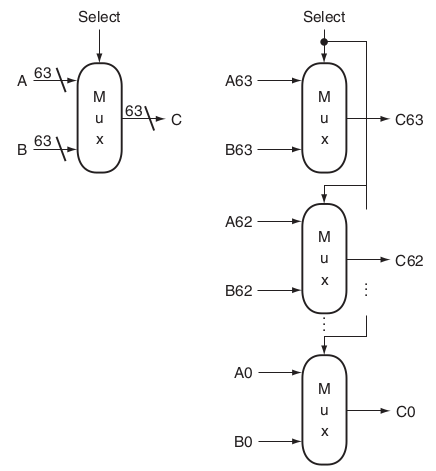
\includegraphics[height=3.5in]{mux_bits.png}
	\caption{An array of 1-bit multiplexers to select from two 64-bit inputs.}
	\label{fig:mux_bits} 
	\end{center}
\end{figure}

\subsection{Designing a 1-bit ALU}

\begin{figure}[H]
	\begin{center}
		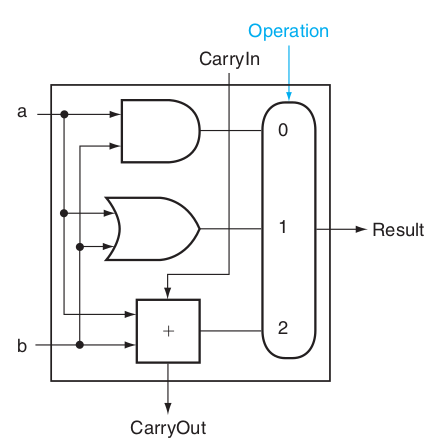
\includegraphics[height=3.5in]{alu.png}
		\caption{A 1-bit ALU design.}
		\label{fig:alu} 
	\end{center}
\end{figure}


We can design a 1-bit ALU that can support the \textit{AND}, \textit{OR}, and \textit{ADD} operations. The diagram is shown in
Figure \ref{fig:alu}. The full discussion of its design and implementation is discussed in the video. The complicated component in this ALU is the Full Adder represented by the rectangle with the plus('+') sign. The VHDL code for the 1-bit ALU is shown below.



\begin{minted}[frame=single,framesep=10pt]{vhdl}
LIBRARY ieee;
USE ieee.std_logic_1164.all;
---------------------------------
ENTITY alu IS
   PORT (a, b, CarryIn : IN STD_LOGIC;
   Operation: IN STD_LOGIC_VECTOR(1 DOWNTO 0);
   Result, CarryOut: OUT STD_LOGIC);
END alu;
--------------------------------
ARCHITECTURE behavioral OF alu IS
   COMPONENT mux_4to1 IS
      PORT (A, B, C, D, S0, S1: IN STD_LOGIC;
      E: OUT STD_LOGIC);
   END COMPONENT;
   COMPONENT and_gate IS
      PORT (A, B: IN STD_LOGIC; C: OUT STD_LOGIC);
   END COMPONENT;
   COMPONENT or_gate IS
      PORT (A, B: IN STD_LOGIC; C: OUT STD_LOGIC);
   END COMPONENT;
   COMPONENT full_adder is
      PORT ( a : IN STD_LOGIC; b : IN STD_LOGIC;
         CarryIn : IN STD_LOGIC;Sum : OUT STD_LOGIC;
         CarryOut : OUT STD_LOGIC);
   END COMPONENT;
   SIGNAL u, v, w, x: STD_LOGIC;
BEGIN
   u1: and_gate port map(a, b, u);
   u2: or_gate port map(a, b, v);
   u3: full_adder port map(a, b, CarryIn, w, CarryOut); 
   u4: mux_4to1 port map(u, v, w, x, Operation(0), 
               Operation(1), Result);
END behavioral;
\end{minted}





\section{Summary}
We discussed some of the combinational elements that are useful in the design of a processor. We also showed the design of a 1-bit ALU that supports a limited set of operations.

\section{Learning Activities}
Download the source codes for this lab then try experimenting by adding more test cases in the testbenches. Submit a PDF document that shows screenshots of your modifications and runs.

\section{Deliverable}
Your final deliverable for this lab is described in the accompanying exercise handout.

%\begin{thebibliography}{9}
%\end{thebibliography}

\bibliographystyle{unsrt}
\bibliography{combi}
\nocite{*}

\end{document}